% !TeX spellcheck = en_GB
% !TeX program = pdflatex
%
% LuxSleek-CV 1.1 LaTeX template
% Author: Andreï V. Kostyrka, University of Luxembourg
%
% 1.1: added tracking and letter-spacing for prettier lower caps, added `~` for language levels
% 1.0: initial release
%
% This template fills the gap in the available variety of templates
% by proposing something that is not a custom class, not using any
% hard-coded settings deeply hidden in style files, and provides
% a handful of custom command definitions that are as transparent as it gets.
% Developed at the University of Luxembourg.
%
% *NOTHING IS HARCODED, and never should be.*
%
% Target audience: applicants in the IT industry, or business in general
%
% The main strength of this template is, it explicitly showcases how
% to break the flow of text to achieve the most flexible right alignment
% of dates for multiple configurations.

\documentclass[11pt, a4paper]{article} 

\usepackage[T1]{fontenc}     % We are using pdfLaTeX,
\usepackage[utf8]{inputenc}  % hence this preparation
\usepackage[british]{babel}  
\usepackage[left = 0mm, right = 0mm, top = 0mm, bottom = 0mm]{geometry}
\usepackage[stretch = 25, shrink = 25, tracking=true, letterspace=30]{microtype}  
\usepackage{graphicx}        % To insert pictures
\usepackage{xcolor}          % To add colour to the document
\usepackage{marvosym}        % Provides icons for the contact details
\usepackage[scale=0.95]{sourcecodepro}
\usepackage{ragged2e}
\usepackage{tabularx} 

\usepackage{enumitem}        % To redefine spacing in lists
\setlist{parsep = 0pt, topsep = 0pt, partopsep = 1pt, itemsep = 1pt, leftmargin = 6mm}

\usepackage{FiraSans}        % Change this to use any font, but keep it simple
\renewcommand{\familydefault}{\sfdefault}

\definecolor{cvblue}{HTML}{304263}

%%%%%%% USER COMMAND DEFINITIONS %%%%%%%%%%%%%%%%%%%%%%%%%%%
% These are the real workhorses of this template
\newcommand{\dates}[1]{\hfill\mbox{\textbf{#1}}} % Bold stuff that doesn’t got broken into lines
\newcommand{\is}{\par\vskip.5ex plus .4ex} % Item spacing
\newcommand{\smaller}[1]{{\small$\diamond$\ #1}}
\newcommand{\headleft}[1]{\vspace*{3ex}\textsc{\textbf{#1}}\par%
    \vspace*{-1.5ex}\hrulefill\par\vspace*{0.7ex}}
\newcommand{\headright}[1]{\vspace*{2.5ex}\textsc{\Large\color{cvblue}#1}\par%
     \vspace*{-2ex}{\color{cvblue}\hrulefill}\par}
%%%%%%%%%%%%%%%%%%%%%%%%%%%%%%%%%%%%%%%%%%%%%%%%%%%%%%%%%%%%

\usepackage[colorlinks = true, urlcolor = white, linkcolor = white]{hyperref}

\begin{document}

% Style definitions -- killing the unnecessary space and adding the skips explicitly
\setlength{\topskip}{0pt}
\setlength{\parindent}{0pt}
\setlength{\parskip}{0pt}
\setlength{\fboxsep}{0pt}
\pagestyle{empty}
\raggedbottom

\begin{minipage}[t]{0.33\textwidth} %% Left column -- outer definition
%  Left column -- top dark rectangle
\colorbox{cvblue}{\begin{minipage}[t][5mm][t]{\textwidth}\null\hfill\null\end{minipage}}

\vspace{-.2ex} % Eliminates the small gap
\colorbox{cvblue!90}{\color{white}  %% LEFT BOX
\kern0.09\textwidth\relax% Left margin provided explicitly
\begin{minipage}[t][293mm][t]{0.82\textwidth}
\raggedright
\vspace*{2.5ex}

\Large Revathy \textbf{\textsc{Venugopal}} \normalsize 

% Centering without extra vertical spacing
\null\hfill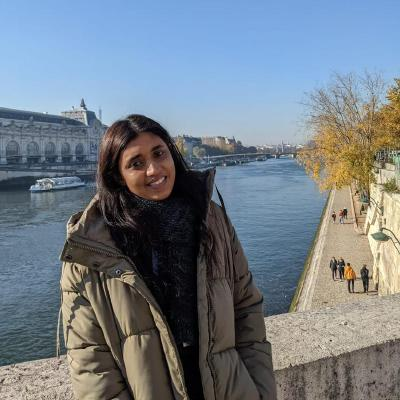
\includegraphics[width=0.80\textwidth]{image.jpeg}\hfill\null

\vspace*{0.5ex} % Extra space after the picture

\headleft{Profile}
Innovative Python developer and open-source contributor with expertise in simulation, automation, and theme development. Main contributor to PyAnsys core team and maintainer for PyDyna. Skilled in building scalable tools, modern web interfaces, and automated processes for engineering workflows.

\headleft{Contact details}
\small % To fit more content
\MVAt\ {\small revathyvenugopal162@gmail.com} \\[0.4ex]
\Mundus\ \href{https://github.com/Revathyvenugopal162}{github.com/revathyvenugopal162} \\[0.1ex]
\Letter\ Lyon, France
\normalsize

\headleft{Personal information}
%Year of birth: \textbf{1861} \\[0.5ex]
Citizenship: \textbf{Indian} \\[0.5ex]
Languages: \textbf{English}~(C1), \textbf{French}~(B1), \textbf{Hindi}, \textbf{Malayalam}
\normalsize

\headleft{Skills}
\small

\vspace{0.5ex}
\textbf{Programming}\\
\vspace{0.5ex}
\begin{tabularx}{\linewidth}{X}
$\cdot$ Python $\cdot$ JavaScript $\cdot$ C \\ $\cdot$ HTML $\cdot$ CSS $\cdot$ Docker \\ $\cdot$ TensorFlow $\cdot$ PyTorch \\ $\cdot$ OpenCV $\cdot$ LaTeX
\end{tabularx}

\vspace{0.5ex}
\textbf{Soft Skills}\\
\vspace{0.5ex}
\begin{tabularx}{\linewidth}{X}
$\cdot$ Problem-solving $\cdot$ Teamwork \\ $\cdot$ Communication $\cdot$ Adaptability \\ $\cdot$ Decision-making $\cdot$ Leadership \\ $\cdot$ Critical thinking $\cdot$ Creativity \\$\cdot$ Emotional intelligence
\end{tabularx}

\vspace{0.5ex}
\textbf{Tools}\\
\vspace{0.5ex}
\begin{tabularx}{\linewidth}{X}
$\cdot$ GitHub $\cdot$ Bitbucket \\ $\cdot$ Sphinx $\cdot$ CI/CD \\ $\cdot$ Jupyter Notebook
\end{tabularx}

\vspace{0.5ex}
\textbf{Languages}\\
\vspace{0.5ex}
\begin{tabularx}{\linewidth}{X}
$\cdot$ English $\cdot$ French
\end{tabularx}

\vspace{1.5ex}


\end{minipage}%
\kern0.09\textwidth\relax%%Right margin provided explicitly to stretch the colourbox
}
\end{minipage}% Right column
\hskip2.5em% Left margin for the white area
\begin{minipage}[t]{0.56\textwidth}
\setlength{\parskip}{0.8ex}% Adds spaces between paragraphs; use \\ to add new lines without this space. Shrink this amount to fit more data vertically

\vspace{2ex}

\headright{Experience}

\textbf{R\&D Engineer,} \textsc{PyAnsys Core Team} \hfill \textit{Ansys (Lyon)} \dates{2022.05--pres.} \\
\begin{itemize}
    \item Main contributor to PyAnsys core team: feature development, code review, release management, and automation tools
    \item Maintainer for PyDyna: simulation modules, automation, and community support
    \item Developed and maintained Ansys Sphinx themes (HTML, CSS, JS, Python)
    \item Built Python-based automation for theme deployment, CI/CD, and build systems
    \item Architected advanced search (Fuse.js, MeiliSearch) for documentation themes
    \item Created responsive, interactive frontend components for engineering UIs
    \item Supported open-source community: onboarding, documentation, and user support
    \item Led cross-functional collaboration with global engineering teams
    \item Applied best practices in software design, testing, and DevOps
\end{itemize}

\is
\textbf{Machine Learning \& Robotics Intern} \hfill \textit{SITIA Robotique (Nantes).} \dates{2021.09--2022.03} \\
\begin{itemize}
    \item Developed Python software for robot vision and obstacle avoidance (TensorFlow, OpenCV).
    \item Implemented real-time algorithms for autonomous navigation.
\end{itemize}

\is
\textbf{Graduate Engineer Trainee} \hfill \textit{BPCL Kochi Refinery (Kerala, India).} \\
\dates{2019.06--2019.08} \\
\smaller{Electrical maintenance, troubleshooting, and repair of electrical equipment.}


\headright{Education}
\textsc{Master of Science in Embedded Systems.} \textit{ESIGELEC, Rouen.}  \dates{2020--2022} \\
\smaller{Embedded systems, software development, machine learning, robotics, computer vision.}

\is
\textsc{Masters degree, Automotive Embedded System.} \textit{Manipal School of Information Sciences.}  \dates{2020--2021} \\
\smaller{Automotive embedded systems, software development, machine learning, robotics, computer vision, IOT, embedded C, Real-time operating systems.}

\is
\textsc{Bachelor of Technology in Electrical and Electronics Engineering.} \textit{College of engineering, Munnar}  \dates{2016--2020} \\
\smaller{Electrical and electronics engineering, power systems, electrical machines, control systems, power electronics.}


\headright{Additional education}

\textsc{Using Python to Access Web Data.}
\textit{Coursera.} \dates{2021} \\
\smaller{Python, web data, web scraping, web services, XML, JSON.}

\is
\textsc{Introduction to Programming Using Python.}
\textit{Coursera.} \dates{2020} \\
\smaller{Python, programming, data structures, algorithms.}

\is
\textsc{Python Data Structures.}
\textit{Coursera.} \dates{2020} \\
\smaller{Python, data structures, algorithms, programming.}

\end{minipage}

\end{document}
